\documentclass{svjour3}                     % onecolumn (standard format)
\usepackage[english, activeacute]{babel} %Definir idioma español
\usepackage[utf8]{inputenc} %Codificacion utf-8
\usepackage[autostyle]{csquotes}
\usepackage[backend=biber]{biblatex}
\usepackage{graphicx}
\usepackage{minted}


\addbibresource{omega-article.bib}
\addbibresource{other.bib}

\graphicspath{ {./images/} }

\begin{document}

\title{ Applying smart policies to dynamic resource managers }

%\titlerunning{Short form of title}        % if too long for running head

\author{ Inigo Mediavilla }
\institute{ UPMC Master STL \at
              \email{imediava@gmail.com}           %  \\
}

\date{\today}

\maketitle

\begin{abstract}
TODO
\end{abstract}

\section{Table of Contents}

\tableofcontents

\section{Introduction}

Scheduling is planning the execution of a set of computations that
are called jobs in an execution environment with a limited amount of
resources.

Fairly recently many factors have boosted a process of
industrialization of the management of software clusters that has
itself increased the relevance of schedulers. 

The popularity of cloud platforms that brings
many companies to opt for not having their own servers, hosting their
services in the datacenters provided usually by the big actors of the
web is one of these factors. 

Another is the burst in the volume of data that companies need to deal
with. This burst has added a new use for clusters initially thought
amongst other things for hosting webservers, databases and distributed
services virtual machines that now can be used to do distributed
parallel processing a discipline that increases the possibility of
manipulating and make sense out of bigger amounts of data.

All those factors added to the increase in the number of their users
has forced the clusters of the big companies to grow almost
exponentially. Bigger clusters mean more complexity, higher resource
consumption and higher economical value of the applications that run
on them. Considering all of that is ease to realise of the importance
of the good utilization of these clusters that depends significantly
on the quality of the schedulers that allocate their resources.


\subsection{Scheduler as the core of a Distributed Operative System}

Scheduling also consists in providing an abstraction layer for
computations to execute their jobs in a distributed environment
without having to manage the distribution of the
computations. As an application that manages the access to
the cluster's resources is actually quite easy to start adding
functionalities to a scheduler to make it the core of a primitive
distributed operative system. If the scheduler is capable of providing
a simple API, it is easy to add other applicative layers on top of
it that can allow a relatively simple programming on top of a
distributed environment.

This movement from simple scheduler, to being the core of a distributed
operative system has already started happening with Mesos whose simple
API has facilitated the creation of frameworks like Aurora \ref{} or
Marathon \ref{} that provide useful primitives for the execution
of applications like load balancing, interservice communication,
or automatic failover.

The implementation of distributed filesystems can also be simplified
thanks to a resource manager as shown by the distributed filesytem
tachyon \ref{} that takes advantage of Mesos primitives. A side effect
of this is that an application running with the resource manager can
take advantage of this distributed filesystems to refer logically to
files stored physically in different nodes of the cluster what means
that schedulers and distributed filesystems complement each other and
represent a big part of our distributed operative system.

Other example of framework that provides operative system primitives
on top of Mesos is Chronos \ref{} that provides simple workflow
management and high level job scheduling and represents a higher
level, distributed alternative to cron.

This primitives themselves greatly facilitate the implementation of
distributed user facing services like distributed web applications
with elastic execution, automatic load balancing and failover (e.g
Marathon + play), distributed build systems (e.g. Jenkins) and of
course the parallel data processing frameworks like Hadoop that were
initially the motivating factor that drove the construction of the
whole distributed environment.

In addition to that this primitives conform the origin of the core of
a distributed operative system a really attractive perspective as data
and users grow quickly. The possibility of a distributed operative
system where data is accessible everywhere in a cluster and services
can run transparently across many nodes and can dynamically adapt
their consumption to the demands of their users constitutes a really
appealing perspective and another reason to consider the relevance of
the schedulers that constitute the very core of the system.


%%- Abstraction over distribution (Parallel processing, Communication
%% interprocesses, Memory, FileSystem)
%%- Failover
%%- Load balancing
%%- Job Isolation

%% Abstraction for the execution of tasks in multiple machines (e.g API)
%%   - Run this in machine X
%%   - Run this in machine X with X CPUs and Y GB Ram
%%   - Communicate with my other task with id X (the cluster should figure out where the task is)
%%   - Autorecover if task fails (if failure is due to the tasks retry n times, if it is due
%%     to a machine find another machine for the task)
    
%%This has allowed to implement on top of the scheduler / resource manager:
%%
%%  - Batch and stream based data processing frameworks (e.g Spark, Hadoop)
%%  - Distributed webs with automatic loadbalancing (e.g Marathon + Play)
%%  - Distributed disk based and memory based file systems (e.g hdfs and tachyon)
%%  - Distributed build systems (jenkins)

%% FIXME: Talk about job isolation

\subsection{Scientific Interest}

This relevance of the scheduling process constitutes a good motivation
for the scientific community to put effort into trying to find the
best scheduling strategies to optimize the utilization of clusters,
and effort that has been eased by the public release of the cluster
traces of many big companies like \ref .Those traces allow anyone
interested in testing improvements to the existing scheduling models
to do it using the information taken from the logs of real
datacenters.

Besides scheduling represents a really interesting problem with many
factors making it a difficult task. Many types of applications can run
in a cluster, with completely different scheduling strategies that the
scheduler needs to support while remaining simple and fast enough to
deal with the increasing size of the cluster and the tighter
scheduling deadlines imposed by recent data processing frameworks.
The scheduler also needs to able to deal with conflicts when many
applications try to use the same resource at the same time and manage
to offer every application a fair share of the resources of the
cluster according to a list of defined criteria. 

Scientifically speaking some of the problems that appear when doing
scheduling are applicable to other fields like microeconomy where
resources need to be shared between different populations. For example
\ref , the algorithm that will be used in our implementation of Omega
has had great implications in the studies that deal with how to share
fairly multiple resources between different individuals in
microeconomy.

Previous approaches to scheduling either have problems to deal with
having to run a diversity of applications, cannot scale when a cluster
grows or don't achieve a high utilization of the resources. Two level
schedulers like Mesos \cite{Hindman10mesos:a} do provide scalability
and flexibility to run different applications but have some
limitations when trying to achieve a good utilization of the resources
of the cluster due to the pessimistic lock that is held with their
offers and can reach deadlocks when two applications do resource
hoarding. Omega \cite{41684} offers a more open model based on
optimistic locking that avoids some inconveniences of the two level
model. However only the model behind Omega has been publicly exposed,
so no available implementation exists that can be used to test Omega
in different contexts. Besides, the Omega paper does not propose an
explanation to how to taken into account bussiness relevance in the
context where frameworks compete for the same resource or how to avoid
problems with \emph{rogue} frameworks apart from a basic notion of
priorities and post-facto monitoring.

%% Be careful cause the simulator could be considered as such implementation

This project will start with a description of the archetypal situation
that a cluster scheduler faces in today's datacenters in section
\ref{sec:archetype} and with a brief comparation in section
\ref{sec:approaches} of how the historical approaches to cluster
scheduling namely centralized scheduling and static partitioning deal
with it, showing their positive and negative aspects. Then we will
study in depth the two main approaches that have been published
recently to deal with dynamic allocation of resources for competing
frameworks in sections \ref{sec:mesos} and \ref{sec:omega} showing
their high level model, their features as well as their advantages and
limitations. 

Finally the most innovative contributions of this project will be
presented. First we will present a prototype implementation of both
models that we'll be schematically explained in section
\ref{sec:implementation} and fully accessible in annex
\ref{annex:implementation} and that will represent in the case of
Omega the first publicly released implementation of the model. Then in
section \ref{sec:businessrelevance} we will fill the gap left by the
paper that describes Omega by explaining how to add two policies
(priorities and DRF) to ensure the consideration of business relevance
with optimistic locking, while section \ref{sec:delayscheduling} will
describe how we have managed to achieve both datalocality and fairness
with DRF thanks to delay scheduling \ref. The last contribution in
sectio \ref{sec:mixed} will be a description of how to emulate
optimistic locking with a two level scheduler, an interesting
technique that opens the door to setup mixed worloads in two level
schedulers.

%% FIXME: Reference to Schwarkpof's paper on why is now the time to
%% build a distributed OS

%% FIXME: correct reference
%In section \ref{FIXME}  we'll describe how our implementation of Omega
%addresses some of this issues through the exposed API.


\section{Archetypal Cluster}
\label{sec:archetype}

Thanks to big companies like Google \ref, Yahoo \ref and Facebook \ref that
have published the traces of their clusters, it is possible today to
have an idea of the activity that happens today in a standard datacenter.
In this section I'll define a characterization of this activity based on
the published traces that I'll use in section \ref{sec:approaches} to 
compare how the more relevant strategies that have been used historically
to schedule jobs in a cluster behave in face of the situation described
by the characterization.

According to Google's traces, cluster's run mainly two group of jobs that
are characterized by their duration. Most jobs last less than 30 minutes
and are mainly MapReduce \ref jobs while a smaller amount of jobs last
more than 18 hours and consume most of the cluster's resources. Yahoo's
and Facebook's traces reveal the same aggregation of tasks between these
clearly differentiated two groups.

Qualitatively speaking the jobs from the first group are mainly parallel
data processing jobs that belong to a myriad of frameworks that includes
MapReduce frameworks like Hadoop, graph processing architectures like
Giraph or Pregel, those specialized for incremental processing like Spark, 
google's Dremel, and Percolator but also MPI jobs. An heterogenous group
of frameworks that uses completely different strategies to scheduler their
tasks. The jobs from the second group require usually high availability and
have more difficult placement constraints what often means that their tasks
take longer to be scheduled.

The traces released by google and publicly accesible at \ref belong to
cluster's with more than eleven thousand machines where rates arrive
at a pace of %%FIXME%% 
per second, however this traces were released in 2011 so
today's numbers have probably increased significantly.


\section{Historical approaches}
\label{sec:approaches}


In the following section we will explain some of the existing models
of cluster schedulers considering their advantages and disadvantages
having into account the criteria introduced in the previous
section. Finally we will introduce the model Omega \cite{41684}
proposed by engineers at google that aims to overcome many of the
limitations of the other approaches.

\subsubsection{Centralized scheduler}

The first schedulers were designed following a monolithic architecture
with a central scheduler taking care of distributing the execution
of jobs across the nodes of the cluster. This design has, at least in
the beginning, the advantage of being simple since there's only one
scheduler assigning resources. The central scheduler controls the
state of the whole cluster, what makes it capable of taking really
good scheduling decisions specially when all jobs have the same
scheduling requirements. 

\begin{figure}[!ht]
  \centering
  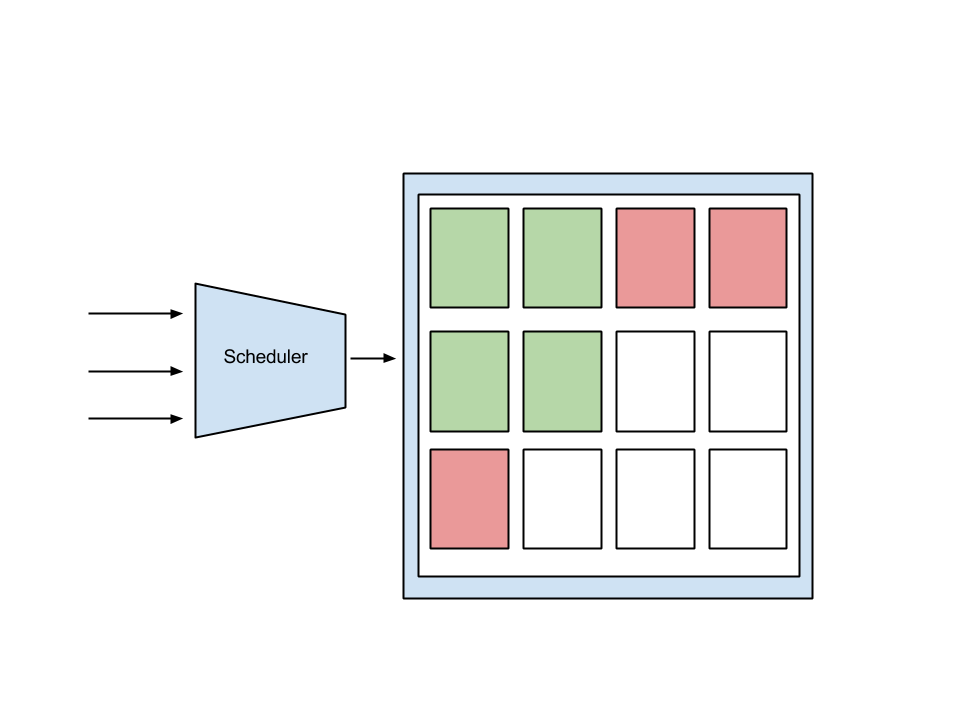
\includegraphics[scale=0.25,natwidth=960,natheight=720]{CentralizedScheduler.png}
  \caption{Centralized Scheduler}
  \label{fig:centralized}
\end{figure}

However this design that is simple and capable of taking good
decisions in the beginning, has many problems as the size of the
cluster increases or as the jobs executed in the cluster
diversify. When the number of jobs to execute increases, the central
scheduler needs to be able to keep with the pace of jobs that are
planned. On top of that a single scheduler represents a single point
of failure. Parallelization can atenuate both problems but just at the
expense of adding complexity and introducing the need for synchronization
between the schedulers.

Above all, for a centralized scheduler it is difficult to adapt
adequately to the heterogeinity of jobs that is executed in today's
clusters \cite{37201}. Trying to define different
scheduling paths for the different types of workloads is difficult
because it requires algorithms to identify the type of a job, and comes
at the expense of the scheduler's complexity. Some schedulers try to
support different policies by implement really complex algorithms
involving different weighting factors that provide rough
approximations of the objectives of every kind of workload. Others
like google's run different scheduling logic for every kind of
workload but it usually implies that users of the scheduler need to
have a really good understanding of the internals of the scheduling
algorithm to be able to optimize the execution of jobs. In both cases
the solution implies an additional layer of complexity to an already
difficult task.

Besides this model requires modifying the code of the scheduler every
time a new type of workload appears. 

Advantages:

\begin{itemize}
  \item Control over the whole cluster. The scheduler is capable of taking good scheduling decisions.
  \item Good cluster utilization
  \item Simplest solution when there's only one framework running in the cluster
\end{itemize}

Disadvantages:

\begin{itemize}
  \item Single point of failure
  \item Doesn't scale. The central scheduler is a bottleneck and
    slower jobs block other jobs that are faster to schedule.
  \item Can't adapt to new frameworks with new policies and needs
  \item Complexity
\end{itemize}

\subsection{Static partitioning}

To overcome the limitations that the previous model had when dealing
with clusters where the are many kinds of jobs with different scheduling
needs, static partitioning allows to split the resources of the cluster
in as many partitions as the kinds of jobs that we want to
treat independently. This strategy is attractive because it allows to
have an optimized dedicated scheduler for every kind while being
relatively simple since every scheduler manages its portion of the
cluster without any risk of conflicts with the others. It was
for a while the model chosen by companies like Yahoo.

\begin{figure}[!ht]
  \centering
  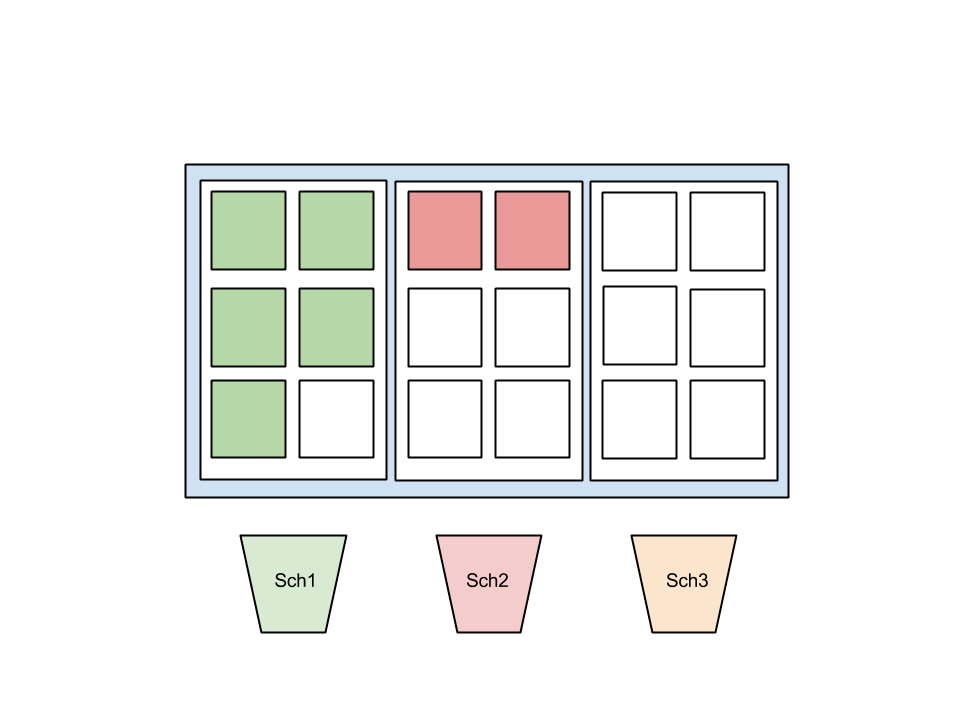
\includegraphics[scale=0.25,natwidth=960,natheight=720]{StaticPartitioning.png}
  \caption{Static Partitioning}
  \label{fig:static_partitioning}
\end{figure}

Nonetheless this strategy's drawback is that since the different 
categories run in different, isolated portions of the cluster the
resources of the cluster are wasted since it is not possible for
a partition to use the resources that another partition is not using.

Advantages:

\begin{itemize}
    \item Simple
    \item Every framework can use their specific scheduler that is specialized
    \item There's no possibility of conflicts between frameworks when
      accessing the resources
\end{itemize}

Disadvantages:

\begin{itemize}
  \item Difficult to decide what is the right partition of the resources
between frameworks
  \item Non-optimal utilization of the resources of the cluster, for example
if one of the frameworks is idle other framework cannot use those
available resources since the repartition is done statically
\end{itemize}

\section{Two-Level scheduler}

\label{sec:mesos}

Two level schedulers give applications, also called
frameworks, the ability to schedule their tasks independently while
having access to all the resources available in the cluster. This
is achieved with an architecture that is based in a master that manages
the cluster's resources and offers them to the frameworks who can accept 
the offers, notifying the master of the tasks they want to run and the
resources they want to run them on, or reject them.

The resources of the cluster are provided by the slaves that register to 
the master at startup providing information about the amount of memory, CPU
and network bandwidth  that they put at master's disposal.  

Frameworks can satisfy their needs (for example data locality \cite{chung_maximizing_2006} ) by 
rejecting the offers that don't interest them and accepting those who do, thus
ensuring per framework needs despite a centralized resource manager. 

When the interests of two frameworks conflict, for example two
frameworks want to run their jobs in the same slave because they both
access the same data, there are techniques to ensure that all
frameworks can have their fair share of the resources they need. In
the case of data processing jobs where tasks don't take long to
execute a technique called delay scheduling \cite{zaharia_delay_2010}
manages to provide good data locality for the tasks without delaying
the execution of the whole job. Nonetheless, when two competing
frameworks use resource hoarding to incrementally acquire resources
before they start a job deadlocks can emerge.

At the cluster level, global policies are enforced by the way that the
master distributes the offers to the frameworks. A cluster manager
like Mesos \cite{Hindman10mesos:a} provides two policies one based on
fairness \cite{AjtaiANRSW1998} and another on strict priorities,
custom policies can also be implemented. However if this policies are
too simple the central scheduler of Mesos can be extended with new
policies.

\subsection{Features}

Since its birth Mesos has experienced a remarkable evolution that have
placed it closer than any other scheduler to providing the API of the
core of the distributed operative system that we described in the
introduction. Some of the features that have helped with this process
are failover and isolation.

Failover on the master is provided with machines that run as backups of the master and
are capable to restore the master's state when it falls. Schedulers and slaves can find
the new master to register to with centralized configuration services like Zookeeper \cite{_apache_????}.

As we have seen in the introduction todays cluster's are made to run a
great variety of jobs belonging to frameworks that may have completely
different objectives. All those frameworks need to work most of the
time isolated from the rest, interferences between frameworks are
exceptions that frameworks ask for explicitly. However it is
impossible or deeply inefficient from the point of view of resource
utilization to run every framework in a different machine to provide
isolation. That means that a scheduler needs means to assign a subset
of the resources of a machine to a job for the execution of its tasks
and ensure that other processes running in the machine cannot
interfere with the tasks running in the subset.

This functionality can already be provided through virtual machines,
but they impose a remarkable overcharge on the processes they run when
compared with the same processes running outside of the virtual
machine, that is the reason why containers where added to
Linux. Containers were initially developed by engineers at Google
under the name of control groups. Control groups are groups of
processes bound by the same rules regarding: \\

\begin{itemize}
  \item Resource limiting
  \item Priorization
  \item Accounting
  \item Control, checkpointing and restarting
\end{itemize}

Control groups work together with another feature of the Linux Kernel
called namespace isolation, that allows to create hierarchies of
groups of processes that cannot see the resources used by other
groups.

The initial advantage of using control groups and namespace isolation when
compared with virtual machines is that processes work in an isolated
environment without the overcharge of virtual machines. However, due
to some of its features, control groups are the perfect ally of a
scheduler when it comes to doing resource allocation since they provide
a really fine granularity for controlling the use of resources such
as CPU use, network bandwith, I/O throughput, memory and file system 
cache they even provide accounting and the possibility of doing
checkpointing and restarting a really useful feature when a scheduler
needs to do preemption over jobs.

Mesos has taken advantage of the features available through linux containers
\cite{_linux_????} to provide its fine grained resource sharing
mechanism as well as isolation and preemption.

\begin{figure}[!ht]
  \centering
  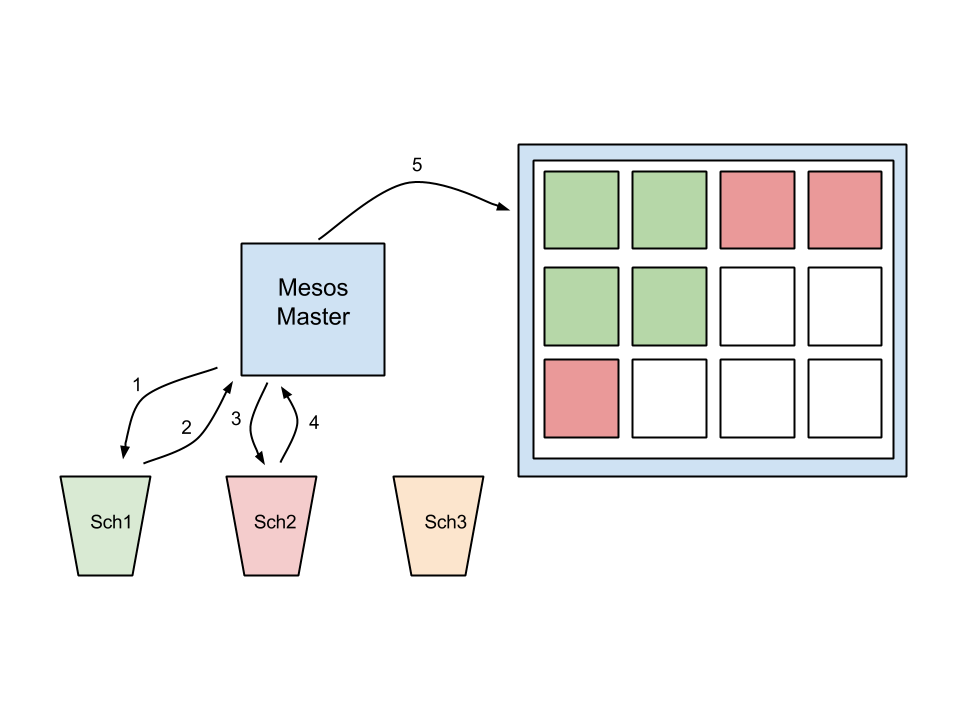
\includegraphics[scale=0.25,natwidth=960,natheight=720]{TwoLevel.png}
  \caption{Two Level Scheduler}
  \label{fig:two_level}
\end{figure}


\subsection{Execution process}

A simple example where we have only one framework that wants to run a 
job formed by a single task will serve to explain all the steps that happen
before a computation can take place in the cluster:

\begin{enumerate}
\item Master starts. One of the candidates is selected as the master and 
the others remain as backup masters that will take the place of the current leader in
case it fails. The leader will start listening to the registration of slaves and 
frameworks.
\item The slaves start. They find the current master through a distributed configuration 
service and they register themselves by notifying the resources the put at the disposal
of the cluster.
\item The framework is launched. To execute its job the framework
  first registers to the master and starts listening to resource
  offers.
\item Since our framework is alone in the cluster, the master makes an offer with
all the resources available to our framework.
\item The framework receives the offer and accepts it. It does so by responding to the
offer with a list of the tasks that it wants to run specifying for every task: how to 
execute the task and what resources will be dedicated to the execution.
The response will only be valid if the resources assigned to all the tasks are a subset
of the resources offered by the master.
\item When the master receives the proposition to run the tasks. It
  allocates the requested resources inside containers in the slaves
  specified in the response and it launches the process to compute the
  task. To be able to run the tasks the slave obviously needs to have
  access to the binaries to run the process what is usually done
  either making the binaries accessible to the whole cluster through a
  distributed filesystem like the Google File System
  \cite{ghemawat_google_2003} or Amazon's S3 \cite{_aws_????} or by
  ensuring manually that the slaves have all the binaries in a public
  accessible folder.
\item Once the computation has finished the slave notifies the master that the resources
are available again so the master can continue offering them to the frameworks.
\end{enumerate}

%% (add diagram over how mesos works?)

Advantages:

\begin{itemize}
  \item
  Really simple central scheduler (master in Mesos terms) that has
  fail-over 
 \item
  Flexible: every framework decides how it schedules its tasks, the
  master only offers resources following fairness 
 \item
  Through offer rejection, frameworks can achieve high data locality
  only accepting offers that correspond to nodes where the data is
  stored. To avoid waiting indefinitely a technique called delayed
  scheduling \cite{zaharia_delay_2010} has proved to achieve high data locality without
  sacrificing job execution time benefiting from the fact that tasks in
  data processing frameworks like Hadoop or MPI are short so resources
  are freed frequently.
 \item Scalability
 \item Specialized for jobs with high chunk and where schedulers don't take
too long. With this kind of job, resources are freed frequently and
every framework gets its fair share of the cluster.
\end{itemize}

Disadvantages:

\begin{itemize}
 \item This kind of scheduling encourages frameworks to demand more
   resources than they actually need in preparation for everything
   they want to run. If a framework wants to run a list of tasks in
   many steps it will demand resources for the whole process even if
   many resources will be idle during most steps.
 \item Difficult to place picky jobs, for example to do gang scheduling
frameworks in Mesos need to do resource hoarding what can lead to
deadlocks
 \item When a framework is offered some resources it
holds the lock for the resource for the time the offer is
available. If a framework hoards the resources or takes a long
time to respond all other frameworks that are actually ready to accept
the offer and execute their jobs will have to wait for the first
framework to respond to the offer.

For example in clusters that run service jobs or jobs with complex
placement constraints that take long time to schedule the performance
of two-level schedulers suffers.

 \item Framework schedulers are written in an indirect style. They
  take actions only when the resources are offered. 
\end{itemize}

\section{Optimistic locking}

\label{sec:omega}

Another approach to cluster scheduling that tries to overcome some of
the limitations of the pessimistic locking of two-level schedulers is
the optimistic locking approach proposed by Google's Omega
scheduler.

The idea behind Omega is to make the state of the cluster available to
every scheduler through a data structure that its called cell
state. When one of the frameworks wants to run a job in the cluster it
tries to commit a lock for the resources needed to run the job's
tasks. If the resource has already been taken by another framework
since the last update, the framework receives the updated version of
the cluster and it can retry a commit of available resources. With
this approach every scheduler has an overall view of the cluster what
allows them to make better scheduling decisions while having a
mediation mechanism when two frameworks want to commit for the same 
resources.

\begin{figure}[!ht]
  \centering
  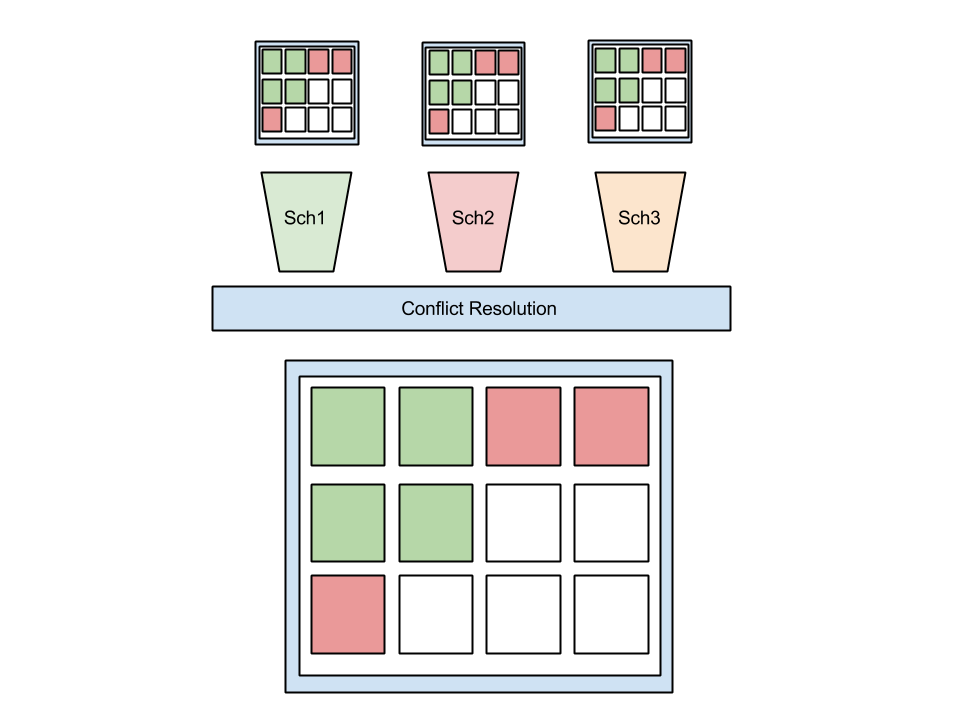
\includegraphics[scale=0.25,natwidth=960,natheight=720]{Omega.png}
  \caption{Omega Scheduler}
  \label{fig:omega}
\end{figure}

Since with this approach the state of the cluster is publicly exposed all the
time for any framework to see, many of the problems that stem from the 
pessimistic locking nature of two level schedulers are avoided.  Frameworks
that take a long time to schedule are no longer a problem since they don't
hold any lock over any resource while they're taking the decision. Besides,
frameworks waiting for an offer no longer have to wait for their turn if they
have a task ready to schedule, they can request the resources as soon as they
know what resources they need and what tasks they will run on them. Frameworks
that don't have any task to run at the moment don't make other frameworks wait
and don't need to worry about responding negatively to offers, they can just
focus on the core of their activity.

Besides, the centralized model behind Omega is way simpler than the
model based on offers used by Mesos. In its basic version, Omega
represents just a thin layer that manages conflict resolution for
concurrent access to cluster's resources. This simplicity makes it
easy for the implementation of a scheduler based on the Omega model to
scale to bigger clusters or higher task interarrival rates.

However, the freedom that the Omega provides for frameworks to
allocate resources in its basic version comes with a drawback when
comparing it with the two level model. While in the two level model,
the master manages what resources are offered to what framework, in
its basic version Omega only accepts or rejects framework's demands
based on wether the resources are available or not.  Therefore Omega
have no way to enforce that the repartition of resources between
frameworks is fair, or that higher priority tasks don't have to wait
for lower priority tasks.

\subsection{Omega Limitations}

In its simplest version Omega was implemented without incremental
resource allocation for tasks and without fine grained resource
management just like the first version implemented for Omega in
[ref]. This version had limitations ...

But even with incremental resource allocation and fine grained
resource management Omega has some limitations, specially as the
cluster ``utilization'' grows and the possibility for conflicts
increases. When dealing with conflicts between tasks there are some
factors to consider:

 \begin{itemize}
   \item (Task duration)If the tasks that conflict (or just the one that is
   running) take minutes to finish, seconds or milliseconds If the
  \item Tasks have different priority levels If the tasks are allowed to be
  preempted or not (if they have high availability requirements they
  can't *Note1*)
 \end{itemize}

When frameworks want to schedule tasks in the cluster they could
either specify the required machines or allow to fallback to the given
amount of resources without considering specific tasks. It's important
that in the case where the cluster provides a fallback mechanism this
should be as simple as possible (for example just taking any other
free machine).


\section{Omega implementation}
\label{sec:implementation}

The paper \ref{} proposed an interesting model to do cluster
scheduling based on optimistic locking that overcomed some of the
limitations of pesimistic locking adopted by two level schedulers like
Mesos. However this paper didn't bring the public release of an
implementation of a scheduler following the premises of the
model. 

This section will present a prototype implementation of a simplified
scheduler based on the Omega model. We will start by describing the
domain model of cluster scheduling that is shared both by our
implementations of Mesos and Omega. Then we will describe the core of
the scheduling mechanism of Omega and compare it with the core of
Mesos what will serve us to see the similarities and differences
between both approaches.

\subsection{Scheduling Domain}

The main concepts behind the domain of scheduling are:

\begin{description}
  \item[Cluster] \hfill \\
  Represents all the available resources available for the frameworks
  to run computations in the environment. This datatype contains the
  resources that are currently avalaible and that can be used to
  schedule tasks, the frameworks that are currently registered as well
  as a list of channels that are used by frameworks to make demands of
  resources for tasks, register or unregister themselves for the
  cluster and notify of finished tasks and therefore released resources.
  \item[Framework] \hfill \\
  Represents an application that will execute computations
  distributedly. It encapsulates a list of tasks that the application
  wants to run with the resources the tasks need and takes care of
  talking with the scheduler to tell him about the tasks it wants to
  run or accepting or refusing offers in the case of Mesos.
  \item[Resources]
  Resources are just a representation of the computational power that
  a cluster offers to run tasks. Our implementation contains only the
  number of CPUs and memory units but other schedulers offer control
  over the I/O or the network bandwith. \\

  An initial implementation of the scheduler represented the resources
  of the cluster as a whole, without specifying what slaves the
  resources belonged to. However this implementation didn't account
  for the tasks' needs to run in a specific node due to the need of
  datalocality. The last implementation called full omega considers
  resources belonging to the slaves and not to the whole cluster this
  way taking into account datalocality.
  
  An interesting property of this datatype is that as resources are
  freed and liberated by tasks resources need to be added and
  substracted what defines an arithmetic of resources where the
  addition represents a monoid.
  \item[Task] \hfill \\
  Is a computation that a framework needs to execute to fulfil its
  objectives. Depending on the implementation the task may be
  responsible of notifying the scheduler when it finishes and its
  resources can be freed.
  \item[Demand] \hfill \\
  A demand represents a task to execute and the resources that are
  needed to execute it. In addition to that, a demand  carry the
  name of the framework that created it what is useful when the
  scheduler needs to apply ordering to demands that is based on the
  framework that made them.

\end{description}

\subsection{Scheduling Core}

In this section we will present the core of the scheduling mechanism
for our prototypes of Omega and Mesos, we will explain how they work
and we will compare them to see the difference between the approaches
of the two models.


\begin{figure}[!ht]
\centering
\begin{minted}[mathescape,
               linenos,
               numbersep=5pt,
               gobble=2,
               frame=lines,
               framesep=2mm]{clojure}
    (defn omegaIter
      [sorting]
      (fn [cluster]
        (let [finishedCh (cluster/getFinishedCh cluster)
            demandsCh  (cluster/getDemandsCh cluster)
            events  (channel/readAll [finishedCh demandsCh])
            demands (channel/belongingTo events demandsCh)
            finishedTasks (channel/belongingTo events finishedCh)
            finishedRes (map task/getResources finishedTasks)
            resourcesFreed (reduce resources/plusResources finishedRes)
            cluster (cluster/addResources cluster resourcesFreed) ]
            (reduce cluster/tryCommitDemand {:cluster cluster :logs []} 
                                               (sorting cluster demands)))))

\end{minted}
\caption{Core of the Omega Scheduling algorithm}
\label{fig:omega-implementation}
\end{figure}

As we can see in figure \ref{fig:omega-implementation} the core of the
scheduling algorithm for Omega is a really simple piece of code that
listens to all finished tasks and to all demands from the
frameworks. It uses the notifications of finished tasks to update the 
list of available resources from the cluster. Then it sorts the
demands with a sorting algorithm that is passed to the function, what
allows to plug the desired sorting algorithm. In most tests, the
default sorting algorithm is a FIFO but thanks to this parameter the
tests that verify that the fairness algorithm works properly only need
to modify the sorting parameter to take the DRF algorithm.

The function \emph{tryCommitDemand} only takes a demand and verifies
if the resources requested by the demand are available, if they do it
substracts the resources from the cluster and runs the task returning
the new state of the cluster. If the resources are not available the
task is not run and the cluster is not modified. In both cases the
demand and its status are logged for notification and tracking
purposes. 


\begin{figure}[!ht]
\centering
\begin{minted}[mathescape,
               linenos,
               numbersep=5pt,
               gobble=2,
               frame=lines,
               framesep=2mm]{clojure}
    (defn offerResources
      [cluster]
      (let [registerCh (cluster/getRegisterCh cluster) 
            finishedCh (cluster/getFinishedCh cluster) 
            frameworks (cluster/getFrameworks cluster)
            resources  (cluster/getResources cluster)
            events     (channel/readAll [finishedCh registerCh])
            finished   (channel/belongingTo events finishedCh)
            registered (channel/belongingTo events registerCh)
            resources (updateResources resources finished)
            frameworks (framework/updateFrameworks frameworks registered [])
            ]
        (reduce offerToAll (cluster/withResources cluster resources) frameworks)))

\end{minted}
\caption{Core of the Mesos Scheduling algorithm}
\label{fig:mesos-implementation}
\end{figure}

As we can see in figure \ref{fig:mesos-implementation} things don't
change much with respect to the omega implementation. The most
important change is that Mesos doesn't deal with demands directly,
instead it makes offers to frameworks that accept them or refuse them
based on the demands they have. The offers are made in the \emph{offerToAll}
method that offers resources to the frameworks one by one and it
receives the responses with the numbers of tasks to run a the
resources they take it updates the state of the cluster.

\begin{figure}[!ht]
\centering
\begin{minted}[mathescape,
               linenos,
               numbersep=5pt,
               gobble=2,
               frame=lines,
               framesep=2mm]{clojure}
    (defn offerToAll
      [cluster fr]
      (let [{demands :tasks newFr :framework}
                  (framework/offeredResources (cluster/getResources cluster) fr)
            resources (map task/getResources demands)
            resourcesTaken (reduce resources/plusResources resources)
            newCluster (cluster/substractResources cluster resourcesTaken)
            newFrameworks (conj (cluster/getFrameworks newCluster) newFr)]
            (doall (for [d demands] ((task/getTask d))))
            (cluster/withFrameworks newCluster (set newFrameworks))))

\end{minted}

\caption{OfferToAll method}
\label{fig:mesos-offerToAll}
\end{figure}

\section{Ensuring business relevance priorization}
\label{sec:businessrelevance}

\subsection{Priorities}

A really simple yet fairly powerful way to consider business needs
when many frameworks want to use the same resources at the same time
is assigning priorities. In the competition for resources, tasks with
higher priorities will always win against lower priority tasks. In the
case where lower priority taks have already their resources assigned
preemption will be used to ensure that the order is respected and that
low priority tasks don't slow down high priority tasks even if this
causes some overhead for the duplicated effort that lower priority
tasks need to do when they're preempted.

In practice this works well because by assigning the higher priority
to the services, that provide the higher business value [ref], we can
ensure their high availability since no other job can preempt them,
and give them exactly the resources they need. Assigning the Lower
priority levels to batch jobs works well because jobs are usually less
important than services but specially because they're more flexible in
the allocation of their tasks, and they deal well with preemption.


%% Idea:


%% Split into small improvements to the things that are not explained in the Omega paper
%% The simulator created can help prove the situation where some of the schedulers doesn't
%% work well and to test some of the improvements' performance.
%%
%% 1. Explaining how to deal with giving preference based on business value
%%    - Show in what situations just mediation for conflicts is not enough
%%       - When some jobs have more priority than others for any allocation (superjobs, e.g services)
%%           (Easy, higher priority jobs can preempt lower priority jobs but not
%%            the opposite - 
%%               -Means that higher priority jobs must behave with responsability 
%%               -Lower priority jobs need to allow preemption (or provide interruptions - can stand-by)
%%               - Can there be any low priority - non-preemptive jobs? why? How to
%%                 deal with that?
%%               - On preemption jobs need to be notified 

%%       - When some jobs have more priority than others for certain allocations (play with
%%         bidding to ensure fairness between same-level frameworks)
%%          - What to base bidding on?
%%             - Job almost finished
%%             - Many other tasks depend on one
%%             - Lower bidding for extending the resources dynamically
%%       - What jobs allow preemption and what jobs don't?
%%
%%   1.1. How can monitoring ensure a good use of the cluster and the fairness provided
%%        by policies?
%%       - Show on simulations of how good and bad fairness levels can be detected and
%%         what can cause a bad fairness level (e.g rogue frameworks, faster
%% 
%% 2. How Omega can be improved when two (or many) jobs want to work over the same data 
%%    (e.g in case of conflicts when do they retry, how to optimize that?)

\subsection{Fairness}

Omega overcomes some of the limitations of the other
scheduling strategies, however in it's basic version it doesn't
provide any control mechanism to ensure that the repartition of
resources between the frameworks is fair or to avoid misbehaving
frameworks monopolizing the control of cluster's resources.

This problem has already appeared in the context of cluster scheduling
and the solution most generally accepted is Dominant Resource Fairness
(DRF) \ref[] that has already been applied to the Mesos two level
scheduler. DRF considers that users care about the number of tasks
they're allocated. The number of tasks allocated for a framework
depends itself on dominant resource that is the resource that
relatively demands most from the cluster, said otherwise the resource
that demands a higher proportion of the cluster for a type of
task. The number of tasks allocated to a user depends on the dominant
resource because it is the one that will be relatively allocated most
of the cluster. DRF attemps therefore to give all users an equal
amount of their dominant resources.

To explain DRF I will use the model of a cluster as a simplified
environment already used at \ref where there are $n$ users
$u_{1},u_{2},...,u_{n}$ and the cluster is represented by a vector of
resources $R_{1},R_{2}...,R_{m}$. Each user $i$ has a \emph{demand
  vector} $D_{i}$, which describes its absolute per task consumption,
e.g., $D_{2} = \langle 3, 2, 1 \rangle$ means that user $u_{2}$ tasks
require 3 units of resource $R_{1}$, 2 units of resource $R_{2}$ and 1
unit of resource $R_{3}$. A user is always given resources as
multiples of its demand vector and allocation is denoted as $A =
\langle a_{1},...,a_{n} \rangle$ what means that user $u_{i}$ gets to
run $a_{i}$ tasks, dimensioned according to its demand vector
$D_{i}$. To simplify, scheduling is considered over an infinite task
demand (i.e. $d_{i} = \infty$).

Formally in DRF each user $i$ has a \emph{dominant share} $x_{i}$ ,
which is $i's$ share of its dominant resource, i.e. $x_{i} = max_{j}\{s_{i,j}\}$,
where $s_{i,j}$ is user $i$'s fractional share of resource $j$, where
$s_{i,j} = a_{i}D_{i,j}/r_{j}$.

An repartition of resources is \emph{Pareto efficient} if it's impossible
to find another repartition where at least one user has more tasks
allocated and all the other users have at least the same tasks. In some 
situations pareto efficienty is incompatible with equal dominant resource
allocation between users, for example if a one user's dominant resource
is not needed at all by the others like figure ~\ref{fig:nonpareto} shows. \\

\begin{figure}[!ht]
\centering
$R = \langle 10, 10 \rangle$ \\
$D = \langle \langle 10, 10 \rangle, \langle 0, 1 \rangle, \langle 0, 1 \rangle \rangle$ \\
\caption{Non pareto efficient equal dominant resource allocation}
\label{fig:nonpareto}
\end{figure}

Then $A = \langle 5, 5, 5 \rangle$ would equalize dominant resource
allocations but it would not be Pareto efficient. Therefore DRF is computed
iteratively with the algorithm described by: \\

\blockquote{Repeatedly allocate one task to the user with minimum dominant
share, for whom there are enough resources to allocate another task.} \\

The allocations obtained by this algorithm satisfy some of the more
relevant criteria that are related to fairness: \\

\begin{description}
  \item[Pareto Optimality (PO)] Already described in the previous
  section this criterium marks a repartition of resources where
  no more tasks can be allocated to user preserving other users'
  allocations.
  \item[Sharing Incentives]  Users are at least as happy as they
  would be under an equal split of the resources.
  \item[Envy-Freeness] Users can't benefit from swaping their
  allocated resources with other users.
  \item[Strategyproofness] Users cannot gain by misreporting
  their demands.
\end{description}

%%FIXME: Extend that
Besides, DRF supports weighted fair sharing similarly to Lottery
Scheduling. 
%%FIXME: How to extend DRF to deal with data locality

\section {How to achieve locality with a Fairness-based allocation algorithm}
\label{delayscheduling}

As we've seen in the introduction, one of the reasons for the
popularity of clusters is the popularization of distributed data
processing frameworks like Hadoop or Google's MapReduce. One of the
advantages of these frameworks is that they can work on big volumens
of data by replicating the data and making accessible through a
distributed filesystem. Then computations are executed in the nodes
that holds the data, profitting from the fact that programs are much
smaller than data, therefore it's quick to send the program where the
data is stored. In summary, these frameworks profit from a property
that is called data locality \ref[].

When only one framework runs in the cluster it is easy to run every
computation in the node that holds the data, specially since the data
is replicated, so many nodes hold the same block of data. However as
the number of frameworks running in the cluster increases it is more
difficult for a scheduler to assign always the right node to every
task. Besides, as many frameworks compete for the resources, schedulers
start considering fairness as the most important criterium, to ensure
that the different frameworks get their fair share of the cluster.

The problem is that as we've seen with the example of DRF, fairness
algorithms don't take into account data locality considerations. In
general fairness algorithms work by offering the last available
resource to the framework that controls the lower share of the cluster's
resources, independently of the node the framework had asked for. This
could lead to the conclusion that achieving fairness and data locality
at the same time is difficult.

Fortunately Zaharia et. al developed in their paper \ref[] a technique
to avoid this problem called delay scheduling. Delay scheduling is a
simple technique that proposes to wait a given timeout before offering
a task resources from a node that doesn't contain the data the task
will use. To avoid that frameworks wait indefinitively after the
timeout a task will receive resources even if they don't come from the
node the task wanted. If the timeout is well fixed, this techniques
achieves good data locality without compromising fairness in
environments where data is replicated across sufficient nodes and jobs
don't last long, what is the case for most distributed processing
frameworks. 

%%\subsection {Implementing Delay Scheduling in Omega}


\section {Isomorphism between Omega and two-level schedulers}
\label{sec:mixed}

Pesimistic and optimistic locking have both advantages and
disadvantages, sometimes pesimistic locking of resources where
resources are kept by a framework for the duration of an offer is
simpler and more adequate since frameworks holding that kind of offer
know that the resources belong to them and if they run tasks on them
they know those tasks would run and they won't be preempted. We have
already seen the advantages of optimistic locking in terms of
efficiency. However for the moment we had seen optimistic and
pesimistic locking as the two opposite sides of a coin and frameworks
implementing allocations based on either one or the other. In this
section we will see that both two level schedulers and Omega-like
schedulers can provide some support for both kinds of locking.

If we look at it from the point of view of the offers that two level
schedulers like Mesos do, the difference between pessimistic locking
and optimistic locking is that in the first offers for a resource are
unique at a given point in time, only the framework that holds the
offer for a resource can launch a task on it. That is why we say that
this frameworks holds a lock on the resource and we say that the lock
is pessimistic because the scheduler assumes that conflicts can happen
at any time and avoids conflicts to happen by only making an offer for
a resource at a time.

On the other hand if a scheduler like Mesos changes its policies and
starts offering all available resources to all frameworks all the time
and takes care of resolving conflicts only when they happened it would
pass from a pessimistic locking to an optimistic locking policy where
it assumes that conflicts happen rarely and that when they happen it
takes care of them.

\begin{figure}[!ht]
  \centering
  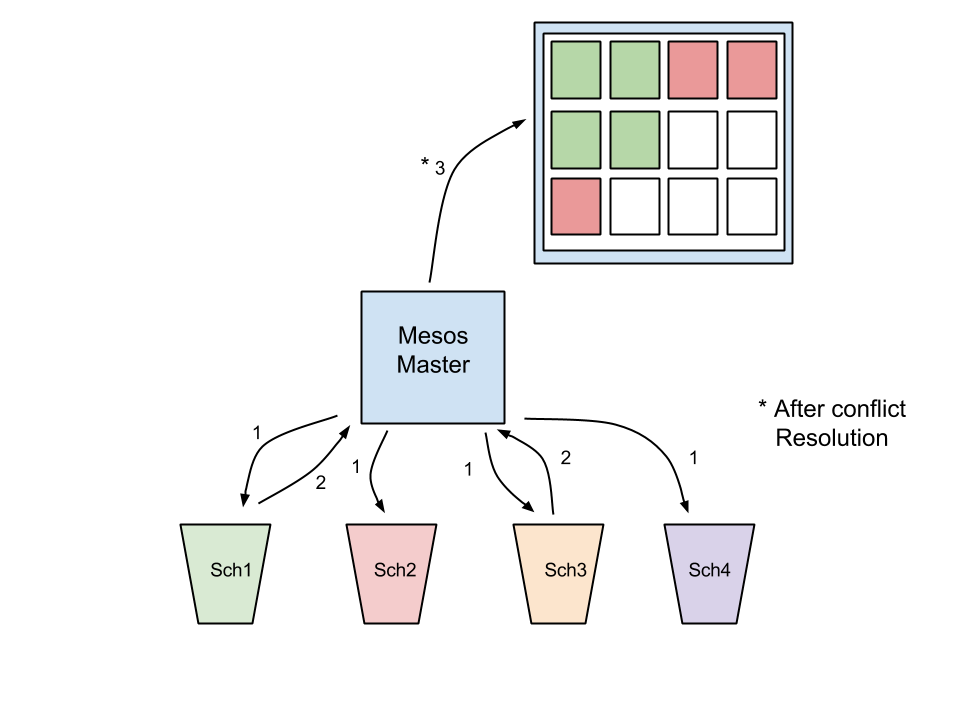
\includegraphics[scale=0.25,natwidth=960,natheight=720]{MesosOptimisticLocking.png}
  \caption{Optimistic Locking with two level scheduler}
  \label{fig:centralized}
\end{figure}

The other way around is also possible if Omega doesn't listen to
demands from all frameworks all the time. If instead it listens to only
one framework at a time and partitions its time between all the
frameworks registered in the cluster then every framework holds the
lock for the available resources of the cluster for the time Omega is
listening to it, working in a similar way a two level scheduler does
when it follows the offer-all strategy.

However both the simulation of optimistic locking with Mesos and the
pessimistic locking with Omega are inefficient. Doing optimistic
locking with Mesos means that all frameworks need to be notified
constantly of all the available resources even if they don't need them
because they don't have tasks to run on them. Pessimistic locking in
Omega implies assigning and arbitrary time per framework that may not
be adequate either demanding loads of negative responses from
frameworks or making them wait when they need resources. The most positive
side of being able to emulate one locking in a scheduler predominantly
based on the other kind of locking is that this avoids having to
choose, allowing mixing, assigning a kind a locking for a subset of
the resources of the cluster and another kind for the rest of the
resources when appropriate.



%% FIXME: Talk about implementation of both in prototype

%%   - How to do optimistic locking with a two level scheduler
%%   - How to do pessimistic locking with Omega (time boxing)
%%   - Mix optimistic and pessimistic locking in a cluster
%%   - Advantages and limitations

\section{Related work}

This project focuses on cluster environments where different
frameworks compete for resources. In this kind of environment the
scheduler is in charge of dispatching resources quick enough
so that the scheduler doesn't become a bottleneck and that every
framework can control the way it schedules its tasks whily ensuring
a good use of the cluster's resources. 

The first two approaches to scheduling namely Centralized Scheduling
and Static Partitioning had troubles ensuring those very first basic
requirements. Centralized Scheduling has the problem that the central
scheduler soon becomes a bottleneck and that frameworks don't have
freedom to schedule freely. Static Partitioning doesn't ensure a good
use of the resources of the cluster.

Leaving aside those two models, the two level model represented by
Mesos \ref and the optmistic approach embodied by Omega \ref are the
two models that provide the basic requirements needed for the type of
cluster that is of interest for this article and that represents a
mayority of the clusters that are found in today's companies. In this
section we will quickly have a look at those models' limitations and
how we have tried to overcome some of them.

As we've seen, the two level model proposes dynamic allocation based on
unique offers that a central scheduler makes to the independent
schedulers of the frameworks. However, this approach shows
inefficiencies since unique offers slow down the allocation of
resources, specially when there are many idle frameworks or some
frameworks take a long time to schedule their tasks.

Omega proposes a model to avoid the problems of the pessimistic
locking of unique offers but it doesn't propose an implementation of
the model. This project proposes a basic prototype implementation 
of Omega and Mesos what gives an idea of the structure that an
Omega-based scheduler can have, how frameworks could communicate with
it and how it compares with a simplified implementation of Mesos.

Besides Schwarzkopf et al. only talk about priorities as a way to
ensure that frameworks with higher business impact get to run their jobs
with a higher preference than less important frameworks and about post
facto monitoring as a supervision technique to ensure that frameworks
make a reasonable use of the cluster. However this is insufficient in
most environments because usually frameworks tend to overdemand
resources and because the basic model with priorities doesn't account
for how to ensure that same priority jobs get similar shares of the
resources of the cluster.

In this project we have explained the way to ensure fairness between
resources introduced by \ref and we have added an implementation of
DRF to Omega, proving that our implementation of Omega can ensure
fairness between same priority frameworks. 

By introducing a fairness-based algorithm like DRF, frameworks lose
the possibility to ensure that their jobs are ran in the slave that
holds the data they're interested in. To avoid this problem our
implementation of Omega uses a technique called delay scheduling \ref
to allow tasks to wait a for the duration of a timeout before
accepting offers from slaves that don't contain copies of the data
that is relevant for them. This way applying the right timeout tasks
achieve a good datalocality without compromising the fair allocation. 

\section{Conclusions and further work}

%\section{Experiments}
%Two-level schedulers have been proven to deal badly with long scheduling decision times and
%when resources are not freed frequently, providing a non-optimal utilization of the resources
%of the cluster.

%Omega doesn't have a clear policy to mediate between frameworks to provide coordination so 
%that the execution can be improved.

%Examples of situations where some global policies can improve the performance of the cluster:

% - A job takes most of the resources but it won't finish soon while other jobs would finish
%   quickly but they are not given the opportunity to use the resources
% - A job that many other jobs depend on is ignored while other job whose execution is less
%   relevant is executed first
%% - A job that can run dynamically adjusting it's size takes resources of other job that needs
%  a fixed amount

%How many of those examples cannot be resolved with priorities? 


\section{Bibliography}


\printbibliography


%% What does the project add?
%% - Retrospective of all models of schedulers (pros/cons)
%% - Implementation of mini Omega
%%   - Solution to implementation problems
%%     - When to do the updates of the cell state?
%%     - How to avoid quickest always wins?
%%     - Failover
%%   - Adding priorities to Omega
%%   - Adding DRF to Omega
%%   - Allowing delayed scheduling with :flexible tag
%% - Explained the isomorphism between two-level scheduler and Omega

%% Future research directions
%%  - Playing game between frameworks thanks to Omega's transparence
%%  (be more concrete)
%%  - Replace DRF + Delay scheduling by a Fairness + Data locality
%%  aware algorithm


%% FIXME:
%% - Higher visibility allows frameworks more flexibility when playing 
%% games and thus to reach a more satisfactory equilibrium. Game theory?
%% - Scheduling is bin packing - Write a remark about this?

\end{document}
